\documentclass[11pt]{article}
\usepackage[margin=1in]{geometry}
\usepackage[T1]{fontenc}
\usepackage{hyperref}
\usepackage{longtable}
\usepackage{array}
\usepackage{enumitem}
\usepackage{relsize, xcolor,xargs, placeins}
\usepackage{float} 
\usepackage{graphicx}


\hypersetup{colorlinks=true,linkcolor=blue,urlcolor=blue}
\setlength{\parskip}{0.5em}
\setlength{\parindent}{0pt}

\title{TAILS Figure-Generating Pipeline Manual}
\date{}

\begin{document}
\maketitle


\FloatBarrier
\begin{figure}[!h]
    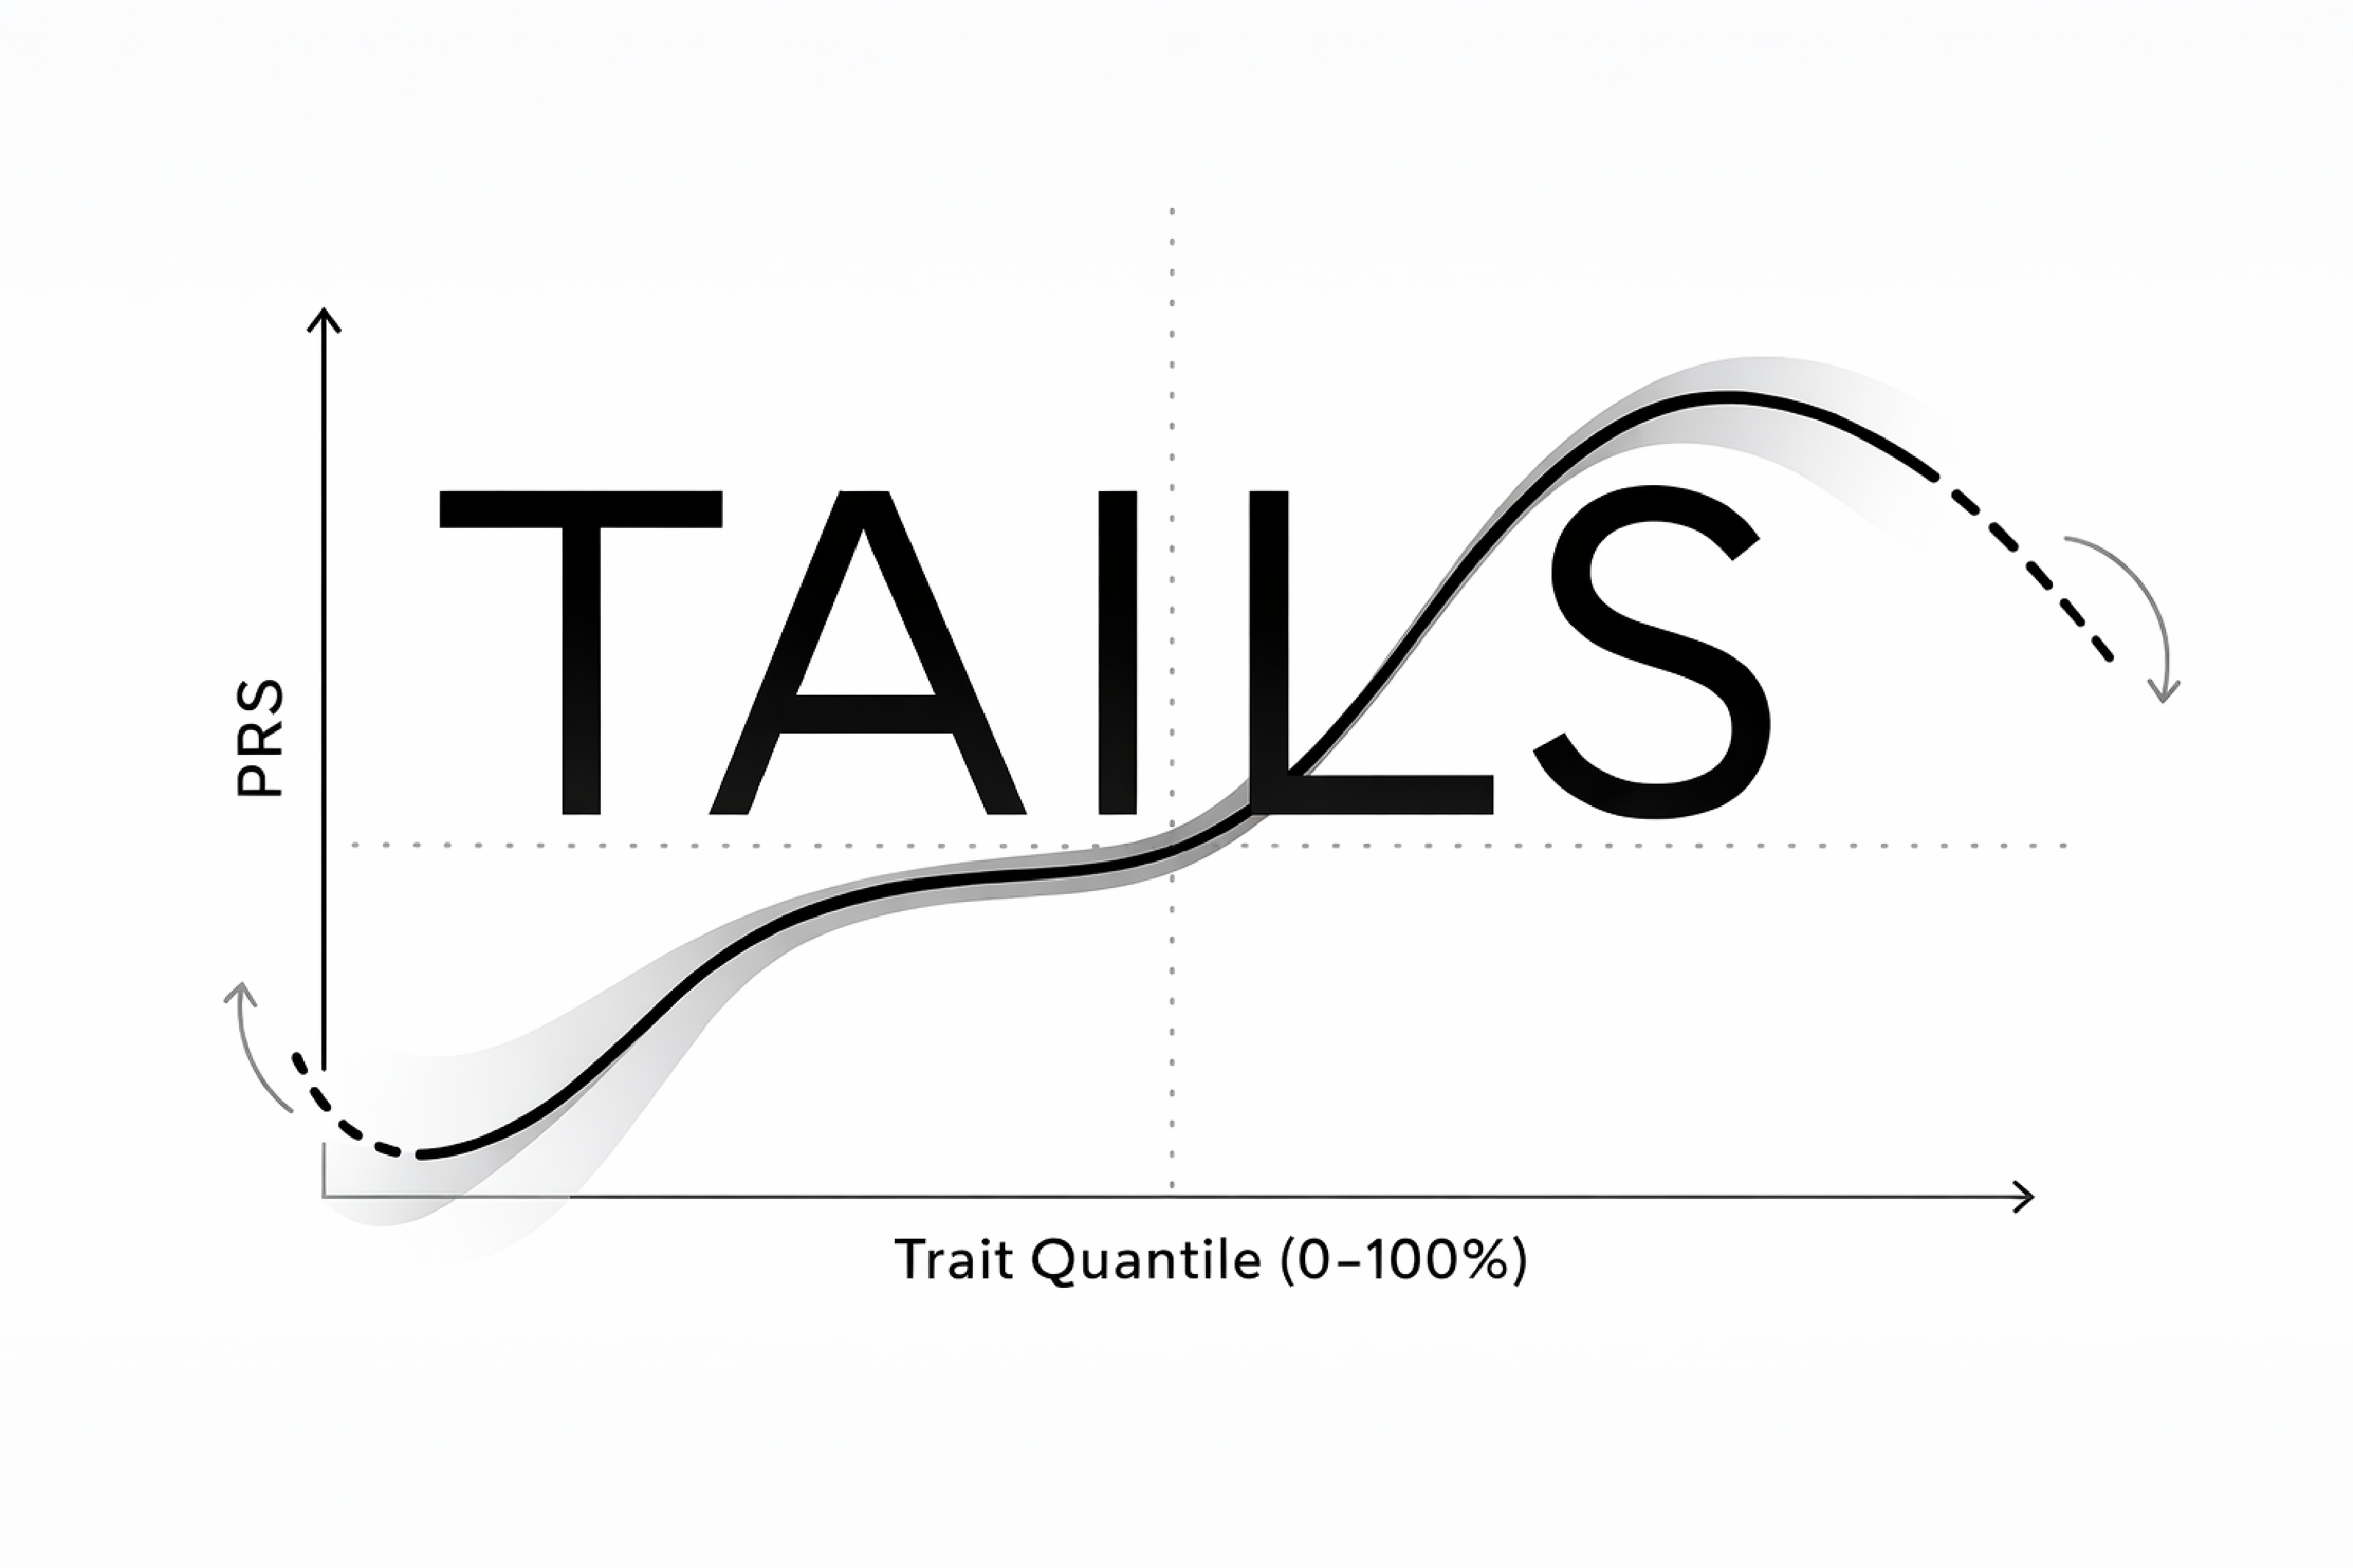
\includegraphics[trim=0cm 0cm 0cm 0cm, clip, width=\linewidth]{tailsLogo.pdf}
\end{figure} \FloatBarrier

\section{Overview}


The TAILS package has two command-line stages:

\begin{enumerate}[nosep]
\item \texttt{tails qc}: merge per-trait QC summaries, inspect available variables, apply filters, and remove highly similar traits.
\item \texttt{tails gen}: generate manuscript figures, extended-data figures, and CSV summary tables from the QC-passed trait set together with packaged analysis outputs.
\end{enumerate}

The intended workflow is sequential: the QC stage writes a filtered trait file, and the figure-generation stage reads that QC-produced file. In the packaged examples, the standard handoff file is:

\begin{verbatim}
output_qc/qc.pass.txt
\end{verbatim}

\section{Package layout}

\begin{longtable}{p{4cm}p{10cm}}
\texttt{code/tails.py} & Main command-line entry point. \\
\texttt{code/src/} & Pipeline source code\\
\texttt{data/} & Bundled trait, QC, and figure-generation inputs. \\
\texttt{docs/} & Documentation. \\
%\texttt{xtended\_latex\_src/} & LaTeX source used to compile the extended-data PDF. \\
\texttt{run\_all.sh} & Example end-to-end script. \\
\end{longtable}

\section{Requirements}

\subsection{System requirements}

\begin{itemize}[nosep]
\item Linux or macOS shell environment
\item Python 3.10+ recommended
\item \texttt{bash}
%\item \texttt{pdflatex} if you want to compile the extended-data PDF in \texttt{xtended\_latex\_src/}
\end{itemize}

\subsection{Python requirements}

The figure-generation code checks for the following Python modules:

\begin{itemize}[nosep]
\item \texttt{matplotlib}
\item \texttt{numpy}
\item \texttt{scipy}
\item \texttt{statsmodels}
\end{itemize}


Example installation:

\begin{verbatim}
python3 -m pip install matplotlib numpy scipy statsmodels 
\end{verbatim}

\section{Top-level commands}

From the package root:

\begin{verbatim}
python3 code/tails.py qc
python3 code/tails.py gen
\end{verbatim}

Useful help commands:

\begin{verbatim}
python3 code/tails.py -h
python3 code/tails.py qc -h
python3 code/tails.py qc load -h
python3 code/tails.py qc filter -h
python3 code/tails.py qc run -h
python3 code/tails.py gen help
\end{verbatim}

Note that \texttt{tails gen -h} is minimal. The generation targets are exposed through \texttt{tails gen help} and through the parsing logic documented below.

\section{QC stage}

The QC stage can be run in two ways:

\begin{enumerate}[nosep]
\item in two steps with \texttt{qc load} followed by \texttt{qc filter}; or
\item in one step with \texttt{qc run}.
\end{enumerate}

\subsection{QC load}

\begin{verbatim}
python3 code/tails.py qc load \
  --in data/namedTraits.txt \
  --qcFiles data/qc/txt/*.txt \
  --out output_qc/qc \
  --showVariables
\end{verbatim}

This command reads the input trait list, merges the QC files, and writes:

\begin{itemize}[nosep]
\item \texttt{output\_qc/qc.merged.txt}
\item \texttt{output\_qc/qc.missing.txt} (if required QC values are absent and \texttt{--allowMissing} was not used)
\end{itemize}

\subsubsection*{QC load arguments}

\begin{longtable}{p{3.2cm}p{10.8cm}}
\texttt{--in} & Input trait file. Required. \\
\texttt{--qcFiles} & One or more QC summary files. Required. \\
\texttt{--out} & Output prefix. Required. This is a prefix, not a directory. \\
\texttt{--showVariables} & Print the available QC/filter variable names and example filters. \\
\texttt{--allowMissing} & Keep traits even when one or more QC files do not supply values. \\
\texttt{--silent} & Suppress progress output. \\
\texttt{--verbose} & Verbose flag exposed by the CLI. \\
\end{longtable}

\subsection{QC filter}

\begin{verbatim}
python3 code/tails.py qc filter \
  --in output_qc/qc.merged.txt \
  --out output_qc/qc \
  --applyFilters "sampleSize-target>50000 h2>0.05 snpmax<0.02 dist-skew<|2| uniq50>2 popQC-pass=True" \
  --dupeFile data/qc/gcorr.mat \
  --configFile data/qc/config.txt
\end{verbatim}

This command applies user-specified filters or the built-in standard filter set, then optionally applies a custom keep/remove configuration and duplicate removal.

Outputs are typically:

\begin{itemize}[nosep]
\item \texttt{output\_qc/qc.pass.txt}
\item \texttt{output\_qc/qc.fail.txt}
\end{itemize}

\subsubsection*{QC filter arguments}

\begin{longtable}{p{3.2cm}p{10.8cm}}
\texttt{--in} & Input file, typically the merged file from \texttt{qc load}. Required. \\
\texttt{--out} & Output prefix. Required. \\
\texttt{--applyFilters} & Space-separated filter string. Mutually exclusive with \texttt{--useStandardFilters}. \\
\texttt{--useStandardFilters} & Apply the built-in standard filter string. Mutually exclusive with \texttt{--applyFilters}. \\
\texttt{--configFile} & Optional custom keep/remove configuration file. \\
\texttt{--dupeFile} & Optional duplicate-correlation file used for deduplication. \\
\texttt{--dupeCutoff} & Deduplication threshold. Default: \texttt{0.99}. \\
\texttt{--dupeTieBreak} & Tie-breaking rule passed to the deduplication logic. Default: \texttt{N}. \\
\texttt{--showVariables} & Show available variables before or during filtering. \\
\texttt{--silent} & Suppress progress output. \\
\texttt{--verbose} & Verbose flag exposed by the CLI. \\
\end{longtable}

\subsubsection*{Standard QC filters}

The built-in standard filter set used by \texttt{--useStandardFilters} is:

\begin{verbatim}
sampleSize-target>50000 h2>0.05 snpmax<0.02 dist-skew<|2| uniq50>2 popQC-pass=True
\end{verbatim}

\subsubsection*{Filter syntax}

Filters are supplied as a space-separated string. Each token has the form:

\begin{verbatim}
VARIABLE OPERATOR VALUE
\end{verbatim}

with no spaces inside a token. Supported operators are:

\begin{verbatim}
<   >   <=   >=   =   !=
\end{verbatim}

Examples:

\begin{verbatim}
h2>0.05
sampleSize-target>50000
popQC-pass=True
uniq50>2
\end{verbatim}

The QC code also supports symmetric absolute-value style thresholds using the \texttt{|value|} syntax. For example:

\begin{verbatim}
dist-skew<|2|
\end{verbatim}

means \texttt{-2 < dist-skew < 2}.

When in doubt, run \texttt{qc load --showVariables} to see the variable names that this particular QC input bundle exposes.

\subsubsection*{Config file behavior}

The optional configuration file passed through \texttt{--configFile} can specify explicit keep/remove actions. The parser recognizes \texttt{KEEP} and \texttt{REMOVE} rules and allows pre/post timing rules. The packaged example uses:

\begin{verbatim}
data/qc/config.txt
\end{verbatim}

\subsection{QC run}

\texttt{qc run} combines \texttt{qc load} and \texttt{qc filter} in one command.

Example:

\begin{verbatim}
python3 code/tails.py qc run \
  --in data/namedTraits.txt \
  --qcFiles data/qc/txt/*.txt \
  --out output_qc/qc \
  --useStandardFilters \
  --dupeFile data/qc/gcorr.mat \
  --configFile data/qc/config.txt
\end{verbatim}

Its arguments are the union of \texttt{qc load} and \texttt{qc filter}.

\section{Figure-generation stage}

The figure-generation stage reads the QC-passed trait file together with bundled analysis files:

\begin{itemize}[nosep]
\item \texttt{--vals}: one or more \texttt{.vals} files
\item \texttt{--pts}: one or more \texttt{.pts} files
\item \texttt{--simPath}: optional simulation directory used by the simulation figures
\end{itemize}

Basic form:

\begin{verbatim}
python3 code/tails.py gen WHICH --in QC_PASS --vals ... --pts ...
\end{verbatim}

\subsection{Figure-generation arguments}

\begin{longtable}{p{3.2cm}p{10.8cm}}
\texttt{WHICH} & Generation target such as \texttt{all}, \texttt{fig2}, \texttt{xtd4}, or \texttt{csv}. Required positional argument. \\
\texttt{--in} & QC-passed trait file. Required. \\
\texttt{--vals} & One or more \texttt{.vals} files. Required. \\
\texttt{--pts} & One or more \texttt{.pts} files. Required. \\
\texttt{--simPath} & Simulation-results directory. Needed for the simulation figure set. \\
\texttt{--dpi} & Figure DPI. Default: \texttt{500}. \\
\texttt{--indexTraits} & Four integer trait IDs used as index traits. Default: \texttt{30810 30070 30020 20015}. \\
\texttt{--out} & Output directory or output prefix for figures/tables. Default: empty string. \\
\texttt{--silent} & Suppress progress output. \\
\end{longtable}

\subsection{Supported generation targets}

The generation parser recognizes the following groups.

\subsubsection*{Aggregate targets}

\begin{longtable}{p{3cm}p{11cm}}
\texttt{all} & Generate all main figures, all extended-data figures, the CSV outputs, and the simulation figure set. \\
\texttt{main} / \texttt{mains} / \texttt{main-figs} / \texttt{figs} & Generate all main figures (1--5). \\
\texttt{xtd} / \texttt{ext} / \texttt{extended-data} / \texttt{sups} & Generate all extended-data figures (1--10). \\
\texttt{csv} / \texttt{csvs} / \texttt{tabs} / \texttt{tables} / \texttt{excel} & Generate the CSV table outputs only. \\
\texttt{sim} / \texttt{sims} & Generate the simulation figure set only. \\
\end{longtable}

\subsubsection*{Single-target forms}

\begin{longtable}{p{3cm}p{11cm}}
\texttt{main1} to \texttt{main5} & Individual main figures. \\
\texttt{fig1} to \texttt{fig5} & Accepted aliases for the main-figure naming convention used in examples. \\
\texttt{xtd1} to \texttt{xtd10} & Individual extended-data figures. \\
\texttt{sup1} to \texttt{sup10} & Accepted supplementary aliases for extended-data figures. \\
\end{longtable}

\subsubsection*{Range forms}

The parser also accepts ranges such as:

\begin{verbatim}
main1-3
fig1-3
xtd2-5
sup2-5
\end{verbatim}

Main-figure ranges must stay within 1--5, and extended-data ranges must stay within 1--10.

\subsection{Main figure-generation example}

\begin{verbatim}
python3 code/tails.py gen all \
  --in output_qc/qc.pass.txt \
  --vals data/trait_data/vals/*.vals \
  --pts data/trait_data/pts/*.pts \
  --simPath data/trait_sims/ \
  --out output_figs/
\end{verbatim}

\subsection{Compiling the extended-data PDF}

After figure generation, the extended-data LaTeX source can be compiled with:

\begin{verbatim}
cd xtended_latex_src
./compileExtendedDocument.sh ../output_figs/
cd ..
\end{verbatim}

This writes:

\begin{verbatim}
xtended_latex_src/extendedData.pdf
\end{verbatim}

\section{End-to-end packaged workflow}

A standard packaged workflow is:

\begin{verbatim}
mkdir -p output_qc output_figs

python3 code/tails.py qc run \
  --in data/namedTraits.txt \
  --qcFiles data/qc/txt/*.txt \
  --out output_qc/qc \
  --useStandardFilters \
  --dupeFile data/qc/gcorr.mat \
  --configFile data/qc/config.txt

python3 code/tails.py gen all \
  --in output_qc/qc.pass.txt \
  --vals data/trait_data/vals/*.vals \
  --pts data/trait_data/pts/*.pts \
  --simPath data/trait_sims/ \
  --out output_figs/

cd xtended_latex_src
./compileExtendedDocument.sh ../output_figs/
cd ..
\end{verbatim}

\section{Outputs}

Typical outputs include:

\begin{itemize}[nosep]
\item \texttt{*.merged.txt}, \texttt{*.missing.txt}, \texttt{*.pass.txt}, and \texttt{*.fail.txt} from the QC stage
\item main-figure PDFs
\item extended-data figure PDFs
\item CSV table exports
\item \texttt{xtended\_latex\_src/extendedData.pdf}
\end{itemize}

\section{Documentation map}

\begin{longtable}{p{4cm}p{10cm}}
\texttt{README.md} & Top-level package overview and quick-start instructions. \\
\texttt{docs/README.qc} & Quick QC commands. \\
\texttt{docs/README.gen} & Quick figure-generation commands. \\
\texttt{docs/tailsManual.pdf} & Full manual. \\
\end{longtable}

\end{document}
